% The first agent session, step by step, with its checks.
% ---------------------------------------------------------------------------
% style.tex --- shared preamble for every figure in book/figures/tikz/
%
% One style for all figures: Latin Modern, thin black lines, a light grey
% fill, and one accent colour used only to mark what is untrusted or wrong.
% Build with scripts/build_figures.sh; see book/figures/README.md.
% ---------------------------------------------------------------------------
\documentclass[tikz,border=6pt]{standalone}
\usepackage[T1]{fontenc}
\usepackage{lmodern}
\usetikzlibrary{arrows.meta,positioning,shapes.geometric,calc,fit,backgrounds}

\hyphenpenalty=10000   % short lines in boxes: ragged, never hyphenated

\definecolor{lightgrey}{gray}{0.92}
\definecolor{accent}{HTML}{9B2D20}

\tikzset{
  every picture/.style={
    line width=0.6pt,
    font=\small,
    >={Stealth[length=5pt,width=4pt]},
    node distance=14pt and 24pt,
  },
  % shapes
  box/.style={draw, rectangle, inner xsep=8pt, inner ysep=5pt,
              minimum height=22pt, align=center},
  grey/.style={box, fill=lightgrey},
  rounded/.style={box, rounded corners=9pt},
  decision/.style={draw, diamond, aspect=2.4, inner sep=1.5pt, align=center},
  group/.style={draw, dashed, rounded corners=5pt, inner sep=7pt},
  % text
  tag/.style={font=\footnotesize, align=center, inner sep=2pt},
  note/.style={font=\footnotesize\itshape, align=center, inner sep=2pt},
  code/.style={font=\small\ttfamily},
  codetag/.style={font=\footnotesize\ttfamily, align=center, inner sep=2pt},
  title/.style={font=\small\scshape, align=center, inner sep=2pt},
  % lines
  arrow/.style={->},
  back/.style={->, dashed},
  thin/.style={line width=0.4pt, gray},
  % the one accent, for what is untrusted, wrong or missing
  bad/.style={accent},
  badbox/.style={box, draw=accent, text=accent},
}

\begin{document}
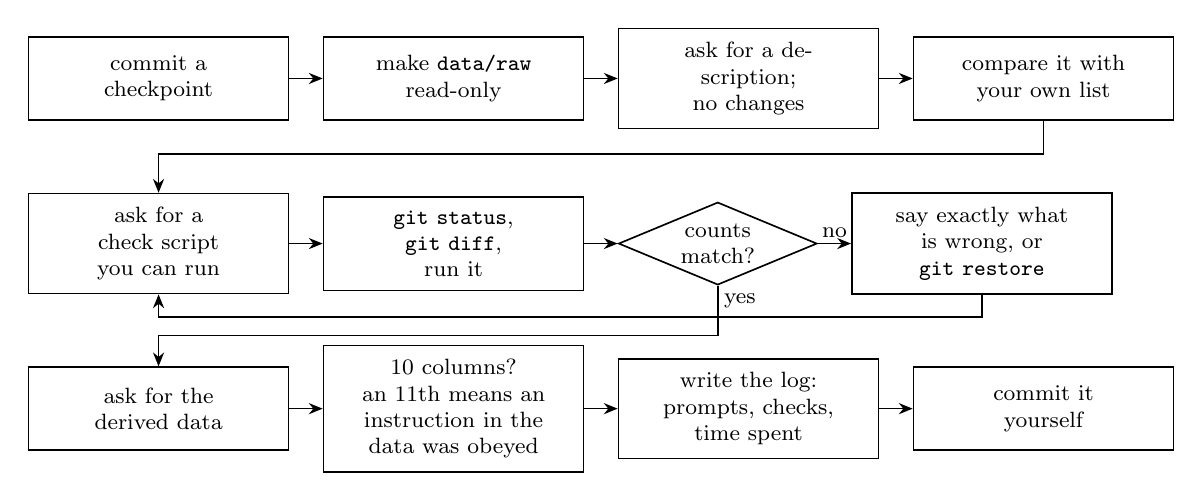
\begin{tikzpicture}[node distance=26pt and 12pt,
                    s/.style={box, text width=78pt, align=center, font=\footnotesize, minimum height=30pt}]
  \node[s] (s1) {commit a\\checkpoint};
  \node[s, right=of s1] (s2) {make \texttt{data/raw}\\read-only};
  \node[s, right=of s2] (s3) {ask for a description;\\no changes};
  \node[s, right=of s3] (s4) {compare it with\\your own list};
  \draw[->] (s1) -- (s2); \draw[->] (s2) -- (s3); \draw[->] (s3) -- (s4);

  \node[s, below=of s1] (s5) {ask for a check script\\you can run};
  \node[s, right=of s5] (s6) {\texttt{git status}, \texttt{git diff},\\run it};
  \node[decision, right=of s6, font=\footnotesize] (s7) {counts\\match?};
  \node[s, right=of s7] (s8) {say exactly what\\is wrong, or\\\texttt{git restore}};
  \draw[->] (s4.south) -- ++(0,-12pt) -| (s5.north);
  \draw[->] (s5) -- (s6); \draw[->] (s6) -- (s7);
  \draw[->] (s7) -- node[tag, above] {no} (s8);
  \draw[->] (s8.south) -- ++(0,-8pt) -| (s5.south);

  \node[s, below=of s5] (s9) {ask for the\\derived data};
  \node[s, right=of s9] (s10) {10 columns?\\an 11th means an\\instruction in the data was obeyed};
  \node[s, right=of s10] (s11) {write the log:\\prompts, checks,\\time spent};
  \node[s, right=of s11] (s12) {commit it\\yourself};
  \draw[->] (s7.south) -- node[tag, right, pos=0.3] {yes} ++(0,-18pt) -| (s9.north);
  \draw[->] (s9) -- (s10); \draw[->] (s10) -- (s11); \draw[->] (s11) -- (s12);
\end{tikzpicture}
\end{document}
